  
    %isolated term
    %#1 - Optional. Space between node and grouping line. Default=0
    %#2 - node
    %#3 - filling color
    \newcommand{\implicantsol}[3][0]{
        \draw[rounded corners=3pt, fill=#3, opacity=0.3] ($(#2.north west)+(135:#1)$) rectangle ($(#2.south east)+(-45:#1)$);
        }
    
    
    %internal group
    %#1 - Optional. Space between node and grouping line. Default=0
    %#2 - top left node
    %#3 - bottom right node
    %#4 - filling color
    \newcommand{\implicant}[4][0]{
        \draw[rounded corners=3pt, fill=#4, opacity=0.3] ($(#2.north west)+(135:#1)$) rectangle ($(#3.south east)+(-45:#1)$);
        }
    
    %group lateral borders
    %#1 - Optional. Space between node and grouping line. Default=0
    %#2 - top left node
    %#3 - bottom right node
    %#4 - filling color
    \newcommand{\implicantcostats}[4][0]{
        \draw[rounded corners=3pt, fill=#4, opacity=0.3] ($(rf.east |- #2.north)+(90:#1)$)-| ($(#2.east)+(0:#1)$) |- ($(rf.east |- #3.south)+(-90:#1)$);
        \draw[rounded corners=3pt, fill=#4, opacity=0.3] ($(cf.west |- #2.north)+(90:#1)$) -| ($(#3.west)+(180:#1)$) |- ($(cf.west |- #3.south)+(-90:#1)$);
    }
    
    %group top-bottom borders
    %#1 - Optional. Space between node and grouping line. Default=0
    %#2 - top left node
    %#3 - bottom right node
    %#4 - filling color
    \newcommand{\implicantdaltbaix}[4][0]{
        \draw[rounded corners=3pt, fill=#4, opacity=0.3] ($(cf.south -| #2.west)+(180:#1)$) |- ($(#2.south)+(-90:#1)$) -| ($(cf.south -| #3.east)+(0:#1)$);
        \draw[rounded corners=3pt, fill=#4, opacity=0.3] ($(rf.north -| #2.west)+(180:#1)$) |- ($(#3.north)+(90:#1)$) -| ($(rf.north -| #3.east)+(0:#1)$);
    }
    
    %group corners
    %#1 - Optional. Space between node and grouping line. Default=0
    %#2 - filling color
    \newcommand{\implicantcantons}[2][0]{
        \draw[rounded corners=3pt, opacity=.3] ($(rf.east |- 0.south)+(-90:#1)$) -| ($(0.east |- cf.south)+(0:#1)$);
        \draw[rounded corners=3pt, opacity=.3] ($(rf.east |- 8.north)+(90:#1)$) -| ($(8.east |- rf.north)+(0:#1)$);
        \draw[rounded corners=3pt, opacity=.3] ($(cf.west |- 2.south)+(-90:#1)$) -| ($(2.west |- cf.south)+(180:#1)$);
        \draw[rounded corners=3pt, opacity=.3] ($(cf.west |- 10.north)+(90:#1)$) -| ($(10.west |- rf.north)+(180:#1)$);
        \fill[rounded corners=3pt, fill=#2, opacity=.3] ($(rf.east |- 0.south)+(-90:#1)$) -|  ($(0.east |- cf.south)+(0:#1)$) [sharp corners] ($(rf.east |- 0.south)+(-90:#1)$) |-  ($(0.east |- cf.south)+(0:#1)$) ;
        \fill[rounded corners=3pt, fill=#2, opacity=.3] ($(rf.east |- 8.north)+(90:#1)$) -| ($(8.east |- rf.north)+(0:#1)$) [sharp corners] ($(rf.east |- 8.north)+(90:#1)$) |- ($(8.east |- rf.north)+(0:#1)$) ;
        \fill[rounded corners=3pt, fill=#2, opacity=.3] ($(cf.west |- 2.south)+(-90:#1)$) -| ($(2.west |- cf.south)+(180:#1)$) [sharp corners]($(cf.west |- 2.south)+(-90:#1)$) |- ($(2.west |- cf.south)+(180:#1)$) ;
        \fill[rounded corners=3pt, fill=#2, opacity=.3] ($(cf.west |- 10.north)+(90:#1)$) -| ($(10.west |- rf.north)+(180:#1)$) [sharp corners] ($(cf.west |- 10.north)+(90:#1)$) |- ($(10.west |- rf.north)+(180:#1)$) ;
    }
    
    %Empty Karnaugh map 4x4
    \newenvironment{Karnaugh}%
    {
    \begin{tikzpicture}[baseline=(current bounding box.north),scale=0.8]
    \draw (0,0) grid (4,4);
    \draw (0,4) -- node [pos=0.9,above right,anchor=south west] {$x_1,x_2$} node [pos=0.7,below left,anchor=north east] {$x_3,x_4$} ++(135:1);
    %
    \matrix (mapa) [matrix of nodes,
            column sep={0.8cm,between origins},
            row sep={0.8cm,between origins},
            every node/.style={minimum size=0.3mm},
            anchor=8.center,
            ampersand replacement=\&] at (0.5,0.5)
    {
                           \& |(c00)| 00         \& |(c01)| 01         \& |(c11)| 11         \& |(c10)| 10         \& |(cf)| \phantom{00} \\
    |(r00)| 00             \& |(0)|  \phantom{0} \& |(1)|  \phantom{0} \& |(3)|  \phantom{0} \& |(2)|  \phantom{0} \&                     \\
    |(r01)| 01             \& |(4)|  \phantom{0} \& |(5)|  \phantom{0} \& |(7)|  \phantom{0} \& |(6)|  \phantom{0} \&                     \\
    |(r11)| 11             \& |(12)| \phantom{0} \& |(13)| \phantom{0} \& |(15)| \phantom{0} \& |(14)| \phantom{0} \&                     \\
    |(r10)| 10             \& |(8)|  \phantom{0} \& |(9)|  \phantom{0} \& |(11)| \phantom{0} \& |(10)| \phantom{0} \&                     \\
    |(rf) | \phantom{00}   \&                    \&                    \&                    \&                    \&                     \\
    };
    }%
    {
    \end{tikzpicture}
    }
    
    %Empty Karnaugh map 2x4
    \newenvironment{Karnaughvuit}%
    {
    \begin{tikzpicture}[baseline=(current bounding box.north),scale=0.8]
    \draw (0,0) grid (4,2);
    \draw (0,2) -- node [pos=0.7,above right,anchor=south west] {bc} node [pos=0.7,below left,anchor=north east] {a} ++(135:1);
    %
    \matrix (mapa) [matrix of nodes,
            column sep={0.8cm,between origins},
            row sep={0.8cm,between origins},
            every node/.style={minimum size=0.3mm},
            anchor=4.center,
            ampersand replacement=\&] at (0.5,0.5)
    {
                          \& |(c00)| 00         \& |(c01)| 01         \& |(c11)| 11         \& |(c10)| 10         \& |(cf)| \phantom{00} \\
    |(r00)| 0             \& |(0)|  \phantom{0} \& |(1)|  \phantom{0} \& |(3)|  \phantom{0} \& |(2)|  \phantom{0} \&                     \\
    |(r01)| 1             \& |(4)|  \phantom{0} \& |(5)|  \phantom{0} \& |(7)|  \phantom{0} \& |(6)|  \phantom{0} \&                     \\
    |(rf) | \phantom{00}  \&                    \&                    \&                    \&                    \&                     \\
    };
    }%
    {
    \end{tikzpicture}
    }
    
    %Empty Karnaugh map 2x2
    \newenvironment{Karnaughquatre}%
    {
    \begin{tikzpicture}[baseline=(current bounding box.north),scale=0.8]
    \draw (0,0) grid (2,2);
    \draw (0,2) -- node [pos=0.7,above right,anchor=south west] {b} node [pos=0.7,below left,anchor=north east] {a} ++(135:1);
    %
    \matrix (mapa) [matrix of nodes,
            column sep={0.8cm,between origins},
            row sep={0.8cm,between origins},
            every node/.style={minimum size=0.3mm},
            anchor=2.center,
            ampersand replacement=\&] at (0.5,0.5)
    {
              \& |(c00)| 0          \& |(c01)| 1  \\
    |(r00)| 0 \& |(0)|  \phantom{0} \& |(1)|  \phantom{0} \\
    |(r01)| 1 \& |(2)|  \phantom{0} \& |(3)|  \phantom{0} \\
    };
    }%
    {
    \end{tikzpicture}
    }
    
    %Defines 8 or 16 values (0,1,X)
    \newcommand{\contingut}[1]{%
    \foreach \x [count=\xi from 0]  in {#1}
         \path (\xi) node {\x};
    }
    
    %Places 1 in listed positions
    \newcommand{\minterms}[1]{%
        \foreach \x in {#1}
            \path (\x) node {1};
    }
    
    %Places 0 in listed positions
    \newcommand{\maxterms}[1]{%
        \foreach \x in {#1}
            \path (\x) node {0};
    }
    
    %Places X in listed positions
    \newcommand{\indeterminats}[1]{%
        \foreach \x in {#1}
            \path (\x) node {X};
    }
    

\section{Ejercicio 2}
\subsection{Introducción}
\newcommand\Tstrut{\rule{0pt}{2.4ex}}
Se tiene una función dada por:

\[
	f(d,c,b,a)=\prod\left(M_{0},M_{1},M_{5},M_{7},M_{8},M_{10},M_{14},M_{15}\right)
\]
\vspace{5mm}
A partir de esto se construyó la siguiente tabla de verdad, completando únicamente los máxterminos de aquellos estados en los que la función valía 0, ya que éstos son los que nos serán de utilidad:

\begin{table}[h!]
	\caption{Tabla de verdad de la función dada.}
	\begin{center}
		\begin{tabular}{|c|c|c|c|c|c|c|}
			\hline
			i  & $d=X_1$ & $c=X_2$ & $b=X_3$ & $a=X_4$ & $f=()$ & $M_i$                                                                          \\\hline
			0  & 0       & 0       & 0       & 0       & 0      & \(X_{1}+X_{2}+X_{3}+X_{4}\)                                                    \\ \hline
			1  & 0       & 0       & 0       & 1       & 0      & \(X_{1}+X_{2}+X_{3}+\overline{X_{4}}\)\Tstrut                                  \\ \hline
			2  & 0       & 0       & 1       & 0       & 1      & -                                                                              \\ \hline
			3  & 0       & 0       & 1       & 1       & 1      & -                                                                              \\ \hline
			4  & 0       & 1       & 0       & 0       & 1      & -                                                                              \\\hline
			5  & 0       & 1       & 0       & 1       & 0      & \(X_{1}+\overline{X_{2}}+X_{3}+\overline{X_{4}}\)\Tstrut                       \\ \hline
			6  & 0       & 1       & 1       & 0       & 1      & -                                                                              \\ \hline
			7  & 0       & 1       & 1       & 1       & 0      & \(X_{1}+\overline{X_{2}}+\overline{X_{3}}+\overline{X_{4}}\)\Tstrut            \\ \hline
			8  & 1       & 0       & 0       & 0       & 0      & \(\overline{X_{1}}+X_{2}+X_{3}+X_{4}\)\Tstrut                                  \\ \hline
			9  & 1       & 0       & 0       & 1       & 1      & -                                                                              \\ \hline
			10 & 1       & 0       & 1       & 0       & 0      & \(\overline{X_{1}}+X_{2}+\overline{X_{3}}+X_{4}\)\Tstrut                       \\ \hline
			11 & 1       & 0       & 1       & 1       & 1      & -                                                                              \\ \hline
			12 & 1       & 1       & 0       & 0       & 1      & -                                                                              \\ \hline
			13 & 1       & 1       & 0       & 1       & 1      & -                                                                              \\ \hline
			14 & 1       & 1       & 1       & 0       & 0      & \(\overline{X_{1}}+\overline{X_{2}}+\overline{X_{3}}+X_{4}\)\Tstrut            \\ \hline
			15 & 1       & 1       & 1       & 1       & 0      & \(\overline{X_{1}}+\overline{X_{2}}+\overline{X_{3}}+\overline{X_{4}}\)\Tstrut \\ \hline
		\end{tabular}
	\end{center}
	\label{table:2.1}
\end{table}

De esta manera, la función está dada por productos de sumas de las variables (máxterminos).

\subsection{Simplificación aplicando álgebra booleana}

Se tiene entonces:
\vspace{5mm}
\begin{dmath}
	f(d,c,b,a)=M_{0}*M_{1}*M_{5}*M_{7}*M_{8}*M_{10}*M_{14}*M_{15}
\end{dmath}
Que es equivalente a:
\begin{dmath}
	f(d,c,b,a)={(X_{1}+X_{2}+X_{3}+X_{4})}*{(X_{1}+X_{2}+X_{3}+\overline{X_{4}})}*{(X_{1}+\overline{X_{2}}+X_{3}+\overline{X_{4}})}*
	{(X_{1}+\overline{X_{2}}+\overline{X_{3}}+\overline{X_{4}})}*{(\overline{X_{1}}+X_{2}+X_{3}+X_{4})}*{(\overline{X_{1}}+X_{2}+\overline{X_{3}}+X_{4})}*
	{(\overline{X_{1}}+\overline{X_{2}}+\overline{X_{3}}+X_{4})}*{(\overline{X_{1}}+\overline{X_{2}}+\overline{X_{3}}+\overline{X_{4}})}
\end{dmath}
\vspace{5mm}
Utilizando la propiedad del álgebra booleana \((x+y)(x+\overline{y}=x)\) sobre los pares de términos \((M_{0},M_{1}); (M_{5},M_{7}); \)\linebreak
\((M_{8},M_{10}); (M_{14},M_{15})\)  se llegó a la siguiente expresión simplificada.
\vspace{5mm}
\begin{dmath}
	f(d,c,b,a)={(X_{1}+X_{2}+X_{3})}*{(\overline{X_{1}}+\overline{X_{2}}+\overline{X_{3}})}*{(X_{1}+\overline{X_{2}}+\overline{X_{4}})}*{(\overline{X_{1}}+X_{2}+X_{4})}
\end{dmath}
\vspace{5mm}


\subsection{Simplificación aplicando mapas de Karnaugh}

\begin{table}[!htb]
	\caption{Mapa de Karnaugh de la función dada.}
	\vspace{5mm} %5mm vertical space
	\begin{minipage}{.45\linewidth}
		\begin{figure}[H]
			\begin{center}
				\begin{Karnaugh}
					\contingut{
						$M_0$,$M_4$,$M_8$, $M_{12}$,
						$M_1$,$M_5$,$M_9$,$M_{13}$,
						$M_2$,$M_6$,$M_{10}$,$M_{14}$,
						$M_3$,$M_7$,$M_{11}$,$M_{15}$}
				\end{Karnaugh}
				\label{table:mapaKarnaughRaw}
			\end{center}
		\end{figure}
	\end{minipage}%
	\scalebox{1.9}{$\boldsymbol{\longrightarrow}$}%
	\begin{minipage}{.45\linewidth}
		\begin{figure}[H]
			\begin{center}
				\begin{Karnaugh}
					\contingut{
						0,1,0,1,
						0,0,1,1,
						1,1,0,0,
					1,0,1,0}
				\end{Karnaugh}
				\label{table:mapaKarnaughsindibujar}
			\end{center}
		\end{figure}
	\end{minipage} 
\end{table}


Nos es de interés para simplificar aplicando mapas de Karnaugh aquellos máxterminos en los que la función vale 0, agrupándolos de a 8, 4, 2 ó 1, según se pueda e intentando que los grupos sean lo más grande posible. Si tomamos 4 grupos de a 2 verticales, como muestra la tabla 
\begin{figure}[H]
	\caption{Mapa de Karnaugh de la función dada.}
	\begin{center}
		\begin{Karnaugh}
			\contingut{
				0,1,0,1,
				0,0,1,1,
				1,1,0,0,
			1,0,1,0}
			\implicant{0}{4}{purple}
			\implicant{5}{13}{red}
			\implicant{15}{11}{green}
			\implicantdaltbaix[3pt]{2}{10}{blue}
		\end{Karnaugh}
		\label{table:mapaKarnaughdibujado}
	\end{center}
\end{figure}

Aquellos seleccionados de manera unitaria en la última columna se tomaron como un grupo de 2.
Con ésto en cuenta, se puede notar lo siguiente de cada pareja:
\begin{itemize}
	\item En el primer grupo de la primera columna, las variables \(X_1, X_2~y~X_3\) valen 0 y no cambian; sí lo hace \(X_4\).
	\item En el segundo grupo, en la segunda columna, las variables que no cambian son \(X_1, X_2~y~X_4\); \(X_1\) vale 0, y \(X_1~y~X_2 \) valen 1, de manera contraria, sí cambia \(X_3\).
	\item En el tercer grupo de ceros, $X_1, X_2~y~X_3$ no cambian y valen 1; notamos que \(X_4\) sí modifica su valor.
	\item En el cuarto grupo en la última columna, $X_1, X_2~y~X_4$ mantienen su valor; con \(X_1\) valiendo 1, y \(X_2,~X_4\), 0; \(X_3\) sí modifica su valor.
\end{itemize}
\vspace{5mm}
\onehalfspacing{Para realizar entonces la simplificación, recordemos que queremos productos de sumas tal que la función sea nula. En el caso del primer grupo, la manera de lograrlo es $X_{1}+X_{2}+X_{3}$, 
	ya que sólo cuando las tres variables valen cero simultáneamente, este término valdrá cero; como $X_4$ cambia su valor no nos es de interés para la expresión.
	De manera análoga para el segundo grupo, podemos lograr que valga cero únicamente con $X_1+\overline{X_2}+\overline{X_4}$. El hecho de negar las variables se debe a que estas valen 1, y se quiere lo contrario.
	Para el tercer grupo, el cero se consigue como $\overline{X_1}+\overline{X_2}+\overline{X_3}$, las tres variables valen 1, por eso se niegan.
	Con el cuarto y último grupo, la nulidad se consigue con $\overline{X_1}+X_2+X_4$.}


\vspace{5mm}
Si se combinan los términos, terminamos con la siguiente expresión:
\vspace{5mm}
\begin{dmath}
	f(d,c,b,a)={(X_{1}+X_{2}+X_{3})}*{(X_1+\overline{X_2}+\overline{X_4})}*{(\overline{X_1}+\overline{X_2}+\overline{X_3})}*{(\overline{X_1}+X_2+X_4)}
\end{dmath}
\vspace{5mm}

ES fácil ver que la expresión es idéntica a la simplificación con el álgebra booleana. Vale agregar que tomando los grupos más grandes posibles al hacer la simplificación con mapas de Karnaugh se llega a la expresión más simplificada posible. Esto verifica también que con el álgebra booleana se pudo reducir la función a su mínima expresión.


\subsection{Circuito lógico resultante}
\subsubsection{Utilizando compuertas AND, OR, NOT.}
Para implementar el circuito lógico, simplemente se tuvo en cuenta la expresión simplificada y se utilizaron compuertas AND, OR, y NOT cuando se requerían.
\begin{center}
	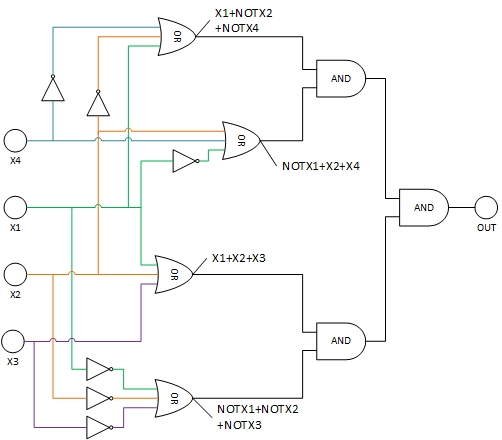
\includegraphics[scale=0.75]{ej2.jpg}
\end{center}

\subsubsection{Utilizando compuertas NOR.}

En este caso se utilizó la compuerta universal NOR para crear las compuertas necesarias (AND, OR y NOT).
De esta manera, se utiliza un número mayor de compuertas, pero universales. El circuito resultante se muestra a continuación:
\begin{center}
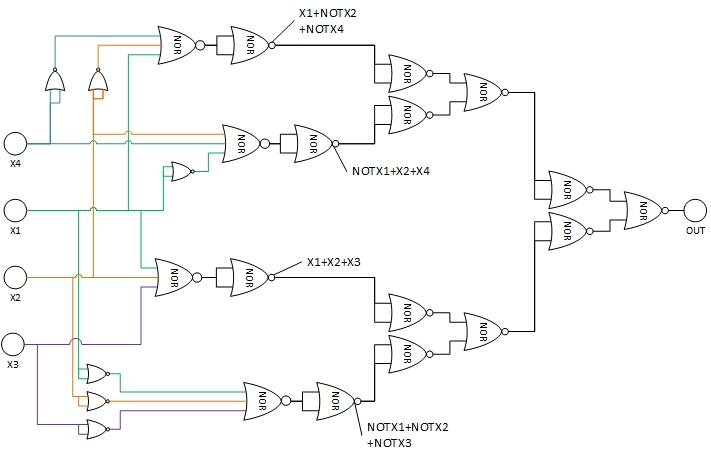
\includegraphics[scale=0.75]{ej2b.jpg}
\end{center}

